\documentclass[acmsmall,screen,review,anonymous]{acmart}

\usepackage{booktabs}
\usepackage{float}
\usepackage{tabularx}
\usepackage{tikz}
\usepackage{xspace}
\usetikzlibrary{arrows.meta,positioning}

\setcopyright{none}
\settopmatter{printfolios=true}
\acmYear{2027}
\raggedbottom
\acmConference[FSE 2027]{ACM International Conference on the Foundations of Software Engineering}{July 12--16, 2027}{Shenzhen, China}
\acmBooktitle{ACM International Conference on the Foundations of Software Engineering (FSE 2027)}
\acmDOI{}
\acmISBN{}
\newcommand{\evar}{\textsc{Evar}\xspace}
\newcommand{\fcr}{\textsc{Fcr}\xspace}
\newcommand{\scr}{\textsc{Scr}\xspace}

\title{Auditing Evidence-Verified Adversarial Review for Code-Review Claims}
\author{Anonymous Author(s)}

\begin{document}
\begin{abstract}
When a code-review agent cites the wrong lines, a second language model can endorse the same plausible mistake. Evidence-Verified Adversarial Review (\evar) instead requires a structured receipt---a file, range, expected observation, falsifier, and optional bounded witness---and makes deterministic verification a precondition for actionability. Unlike benchmarks of open-ended issue discovery, we hold one review claim fixed and ask whether checked evidence justifies acting on it. We compare ordinary adversarial review (AR), textual evidence (AR-Text), and \evar-Hard with matched cases and call budgets. On an untouched temporal holdout derived from ten public review comments, \evar-Hard ties or trails AR-Text; later models and providers do not produce a stable performance ordering. A post-hoc same-row audit then isolates enforcement from information. Among 388 completed \evar-Hard decisions, the final gate changes none because the critic had already seen the verifier outcome and rejected every receipt the gate would reject. Apparent differences from AR-Text therefore mix receipt representation, critic context, and enforcement. Across 1,200 attempts, 1,166 complete, all 34 failures are typed, and all 144 hard-protocol actionable findings have verified supporting receipts. The main contribution is methodological: a deterministic rule at an action boundary is not evidence of a causal gate effect when its signal is already visible upstream. We provide a temporally paired claim-validation task, a judge-free mechanism audit, and a preregistered verification-blind design that identifies enforcement separately from verifier-aware judgment.
\end{abstract}

\keywords{code review, language-model agents, evidence verification, benchmark, reliability}
\ccsdesc[500]{Software and its engineering~Software testing and debugging}
\ccsdesc[300]{Computing methodologies~Natural language processing}
\maketitle

\section{Introduction}

Reviewer-critic systems use a second model call to challenge or refine a first model's answer. Iterative self-feedback and multi-agent debate can improve generation and reasoning \cite{selfrefine,debate}, but textual agreement is not independent evidence. In code review, two agents can converge on the same plausible interpretation of code while both overlook the observation that would falsify it.

Consider a documentation finding from Black pull request 5272 in our holdout. A human reviewer asked that an internal explanation involving \texttt{hug\_power\_op} and cloned leaves be replaced with a concise user-facing changelog entry. The same claim is true at the reviewed commit and false after the merge edit. A textual critic can accept the finding in either snapshot because the wording remains plausible. An evidence receipt must instead identify the exact changelog lines present in that snapshot. The example captures our unit of analysis: not whether a model can discover every issue in a pull request, but whether one candidate finding deserves to cross an actionability boundary.

\evar changes the acceptance path. A reviewer submits a structured evidence receipt; a deterministic verifier checks a source location or executes a bounded witness; and only a verified receipt can become actionable. We first compare end-to-end decision quality, then audit whether the final gate itself changes decisions rather than inheriting behavior already induced by verifier-aware criticism.

We organize the study around four research questions:
\begin{description}
  \item[RQ1 (decision quality).] Does deterministic evidence verification reduce unsupported actionable findings without an unacceptable loss of supported findings?
  \item[RQ2 (gate mechanism).] When receipt, verifier output, and critic decision are fixed, does the final hard gate change actionability?
  \item[RQ3 (model sensitivity).] Does the safety--retention operating point persist across model capability and provider families?
  \item[RQ4 (auditability).] Which protocol failures and acceptance invariants become mechanically observable?
\end{description}
The distinction between decision quality and auditability matters throughout the paper. A receipt can be mechanically valid yet irrelevant to the claim, and a protocol can be easier to audit without producing a better \fcr/\scr pair.

Our contributions are deliberately about claim validation and mechanism identification, not a new open-ended review generator:
\begin{enumerate}
  \item \textbf{Claim-validation task and benchmark:} we fix a human review claim and pair the exact reviewed and merged snapshots, controlling claim wording while changing whether the repository supports it;
  \item \textbf{Auditable acceptance protocol:} a structured receipt and deterministic verifier expose what observation was checked, why it failed, and which rule allowed a claim to become actionable;
  \item \textbf{Causal mechanism result:} matched experiments and a same-row replay show that the reported hard gate is observationally redundant after verifier-aware criticism, separating an auditable invariant from an accuracy or enforcement effect;
  \item \textbf{Identifiable follow-up and artifact:} a preregistered verification-blind arm isolates enforcement without another stochastic call, while frozen inputs, transcripts, manifests, and judge-free audits preserve every one of 1,200 attempts, including failures.
\end{enumerate}

The contribution is therefore not the general idea of using tools or deterministic checks around an LLM. Prior systems already use external feedback and action-boundary rules. The new research question is whether a checked evidence receipt changes the actionability of a \emph{supplied code-review claim}, and whether that effect remains after separating the information shown to the critic from the rule enforced afterward.

\section{Related Work}

\subsection{Reflection, critique, and debate}

Self-Refine uses model-generated feedback to iteratively improve a model's output \cite{selfrefine}. Reflexion incorporates linguistic feedback into an episodic memory rather than updating model weights \cite{reflexion}. Multi-agent debate has similarly improved reasoning and factuality through textual deliberation \cite{debate}. These methods motivate the AR baselines but do not, by themselves, make agreement independent evidence. The same model family can reproduce a shared misconception across reviewer and critic roles. Ji makes this limit concrete for groundedness judgments: a homogeneous three-agent panel changes accuracy by between $+8.5$ and $-4.4$ points relative to a single judge across six fact-verification benchmarks, and the author notes that such differences characterize complete systems rather than isolating debate itself \cite{more-debate}. The same attribution problem reappears in our gate analysis.

Refute-or-Promote is the closest adversarial-review design in software security \cite{refute-promote}. Its pipeline promotes LLM-found defect candidates only through adversarial kill-gates, cold-start reviewers, and a cross-model critic, and it reports a case in which reviewers unanimously endorsed a non-existent padding oracle until an empirical validation gate rejected it. That practitioner study targets open-ended discovery and reports pipeline outcomes rather than a matched protocol comparison. \evar studies the same false-consensus risk under controlled conditions: one supplied claim, a matched call budget, and a deterministic receipt check whose information and enforcement roles can be separated.

Prior work also questions whether intrinsic self-correction is reliable without external feedback. CRITIC couples model critique to tool interactions and reports gains across question answering, program synthesis, and toxicity reduction \cite{critic}. \evar adopts the external-feedback premise but narrows both the task and the acceptance rule: the system judges a pre-specified code-review claim, and a deterministic receipt check is a necessary gate rather than optional context for another revision. More recently, \emph{Reason Less, Verify More} places deterministic, read-only gates immediately before policy-sensitive tool writes and demonstrates gains when tools do not enforce their own domain policy \cite{reason-less}. That work establishes the value of action-boundary enforcement in a general agent setting. \evar instead studies whether code evidence supports one review claim and exposes a different causal pitfall: when verifier status is already shown to an upstream critic, applying it again at the boundary need not change any decision.

Negative evidence is equally relevant. Huang et al. find that intrinsic self-correction can leave reasoning unchanged or make it worse when no reliable external signal is available \cite{huang-self-correct}. In software tasks, Crupi et al. report that even strong LLM judges frequently misclassify code correctness and summary quality \cite{crupi-judge}, while Moon et al. show that superficial changes to otherwise equivalent code systematically perturb judge verdicts \cite{moon-code-judge}. GroundEval responds to similar judge failures in stateful agent evaluation by scoring what an agent actually searched, fetched, and cited; it reports a response that frontier judges rated highly although the agent never retrieved the artifact its answer depended on \cite{groundeval}. These results motivate our separation of textual criticism, deterministic verification, and semantic ground truth.

\subsection{Tool-using software-engineering agents}

SWE-agent shows that the interface between a model and a computer materially affects software-engineering performance \cite{sweagent}. Executable feedback can reveal failures that are invisible in a textual conversation, but unrestricted agent execution also introduces a large design surface. \evar uses a deliberately narrow interface: structural source checks or a shell-free verification process launched from the benchmark fixture under a timeout. This makes the acceptance boundary easier to audit, at the cost of incomplete coverage for repository-scale semantic claims. The current code includes a hardened container option for future runs; the experiments reported here used trusted fixtures and the local backend.

\subsection{Code review as a sociotechnical practice}

Modern code review is not reducible to defect detection. Interviews at Microsoft identify knowledge transfer, alternative solutions, and team awareness alongside finding defects \cite{bacchelli-bird}; Google's review process likewise emphasizes a lightweight, tool-mediated practice embedded in development rather than a standalone classifier \cite{sadowski}. This broader view constrains our claims. FCR and SCR measure the fate of a supplied technical claim, not whether a generated comment is timely, understandable, or useful to a team. Industrial studies of deployed automated review systems further show why adoption and workflow outcomes require separate measurement \cite{automated-practice,rovodev}. We therefore treat developer utility as future work rather than inferring it from benchmark accuracy.

\subsection{Automated code review and benchmarks}

Early neural approaches learned review-time code transformations and comment-conditioned refinements \cite{tufano-automating}. Later work showed that task-specific T5 pre-training improves those automation tasks \cite{tufano-pretrained}, while CodeReviewer jointly targets change-quality estimation, comment generation, and refinement \cite{codereviewer}. These systems ask whether a model can generate or implement review feedback. Our task begins later: a candidate claim already exists, and the system must decide whether the repository snapshot supports actionability.

A recent survey of 99 code-review studies organizes the area into 18 tasks \cite{review-survey}. Empirical audits also expose limitations hidden by aggregate generation scores: Tufano et al. characterize where review-automation systems succeed and fail through manual inspection \cite{tufano-strengths}, and Liu et al. find that vague or non-actionable training comments remain after conventional cleaning \cite{too-noisy}. That heterogeneity and data noise are important here: EVAR is a claim-validation benchmark, not a substitute for issue discovery, localization, comment generation, or developer-utility evaluation.

Hybrid review systems combine learned generation with rule-based analyzers to recover some precision without surrendering broad issue coverage \cite{hybrid-static}. \evar shares the motivation but assigns the deterministic component a different role: it validates the submitted observation and controls actionability; it neither generates a parallel comment nor establishes semantic relevance by itself.

Alert triage offers a close analogue outside code review. Xiong and Zhang compare Aider, OpenHands, and SWE-agent as filters for static-analysis false positives and find that the strongest configurations remove most false alarms, but that gains depend on the backbone model and vulnerability class and that aggressive filtering can suppress real vulnerabilities \cite{sifting-noise}. That is the same safety--retention tension that FCR and SCR keep separate here.

Software-engineering benchmarks increasingly ground tasks in public development history. SWE-bench uses real GitHub issues and pull requests and demonstrates the need for repository context and executable environments \cite{swebench}. SWE-PRBench evaluates code-review models against pull-request feedback and reports limited detection of human-flagged issues \cite{sweprbench}. Our task is narrower: a candidate claim is given, and the system must decide whether it remains actionable under the supplied repository snapshot.

SWR-Bench makes a complementary choice: it evaluates 1,000 complete pull requests with full-project context and structured ground truth, then asks whether generated reviews cover the reported issues \cite{swrbench}. EVAR is smaller and deliberately different. It does not score open-ended issue discovery; it fixes one candidate claim and asks whether that claim can cross an auditable evidence boundary. That trades breadth for a clean test of false consensus and lets us report why a finding was accepted, rejected, or mechanically unverifiable. A future larger benchmark should combine EVAR's receipt-level audit with the PR-scale context and manual verification used by SWR-Bench.

c-CRAB derives tests from human pull-request reviews and uses them to judge whether a review agent identified the same issue; existing agents collectively solve about 40\% of its tasks \cite{ccrab}. Executable validation of review content is close to \evar's behavioral witnesses. The difference is again the unit: c-CRAB tests an agent's discovered issues against held-out tests, whereas an \evar receipt is the reviewer's own falsifiable observation for a claim that is already fixed.

ContextCRBench reaches a different scale, with context-enriched entries for quality assessment, localization, and comment generation \cite{contextcrbench}. Its emphasis on issue context and fine-grained localization reinforces an important external-validity limit here: EVAR's focused excerpts isolate the verification question, but they cannot substitute for evaluating complete pull requests with developer intent.

AACR-Bench provides multilingual, repository-level context and uses AI-assisted, expert-verified annotation to uncover defects beyond the original review record \cite{aacrbench}. This improves the breadth of open-ended review evaluation and makes language and retrieval effects measurable. EVAR controls a different experimental unit: it does not ask a model to find an unknown defect, but tests the support and actionability of a fixed claim under two historical repository states.

Sphinx constructs context-rich PR-review examples, evaluates generated reviews with actionable checklists, and uses those checklists as interpretable training rewards \cite{sphinx}. Its structured verification points are close in spirit to evidence receipts, but the unit and objective differ: Sphinx scores coverage and trains a review generator, whereas EVAR holds one claim fixed and audits the causal path from submitted evidence to actionability.

These comparisons delimit the contribution. SWR-Bench, SWE-PRBench, AACR-Bench, ContextCRBench, c-CRAB, and Sphinx primarily measure discovery, localization, generation, test-validated issue coverage, or checklist coverage. CRITIC and \emph{Reason Less, Verify More} supply the closest mechanism precedents for external feedback and deterministic gates, and Refute-or-Promote the closest adversarial-review pipeline. EVAR occupies their intersection: temporal code-review claim validation with a machine-checked receipt, followed by an explicit test of whether enforcement itself changes the decision. We make no priority claim for deterministic gating in general.

\section{Protocols}

All protocols receive the same candidate claim, task description, repository context, model configuration, and two-call interaction budget: one reviewer call followed by one critic call. The reviewer always returns exactly one schema-constrained receipt. The protocols differ in what happens to that receipt before criticism.

\begin{table}[h]
\centering
\caption{Compared protocols.}
\label{tab:protocols}
\begin{tabularx}{\linewidth}{@{}lXX@{}}
\toprule
Protocol & Evidence handling & Actionability gate \\
\midrule
AR & Reviewer proposes a finding; critic evaluates textually. & Critic returns \texttt{ACCEPT}. \\
AR-Text & Reviewer adds textual evidence when challenged. & Critic returns \texttt{ACCEPT}. \\
\evar-Hard & Reviewer submits a receipt; verifier checks structural or behavioral evidence. & Verifier returns \texttt{VERIFIED} and critic returns \texttt{ACCEPT}. \\
\evar-BlindGate & Same receipt and verifier; result is withheld from the critic. & Emits paired soft and hard decisions (powered follow-up). \\
\bottomrule
\end{tabularx}
\end{table}

Figure~\ref{fig:evar-architecture} situates the protocol choice within the complete data, decision, and audit pipeline.

\begin{figure}[t]
\centering
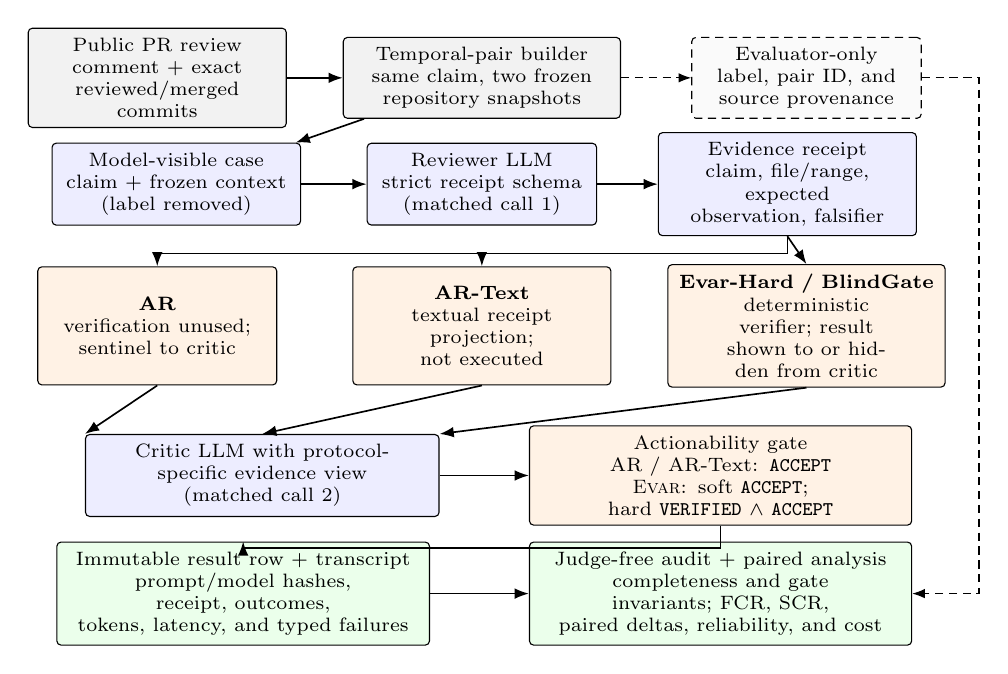
\begin{tikzpicture}[
  x=\linewidth,
  y=1cm,
  box/.style={draw, rounded corners=1.5pt, align=center, inner sep=3.5pt,
              font=\scriptsize, minimum height=8mm},
  provenance/.style={box, fill=black!5},
  model/.style={box, fill=blue!7},
  protocol/.style={box, fill=orange!10},
  artifact/.style={box, fill=green!8},
  hidden/.style={box, densely dashed, fill=black!2},
  flow/.style={-{Latex[length=1.8mm]}, semithick},
  sideflow/.style={-{Latex[length=1.6mm]}, densely dashed, thin}
]
  % Provenance and case construction.
  \node[provenance, text width=.25\linewidth] (source) at (-.34,0)
    {Public PR review\\comment + exact\\reviewed/merged commits};
  \node[provenance, text width=.27\linewidth] (builder) at (0,0)
    {Temporal-pair builder\\same claim, two frozen\\repository snapshots};
  \node[hidden, text width=.22\linewidth] (labels) at (.34,0)
    {Evaluator-only\\label, pair ID, and\\source provenance};
  \draw[flow] (source) -- (builder);
  \draw[sideflow] (builder) -- (labels);

  % Model-visible input and first call.
  \node[model, text width=.24\linewidth] (case) at (-.32,-1.35)
    {Model-visible case\\claim + frozen context\\(label removed)};
  \node[model, text width=.22\linewidth] (reviewer) at (0,-1.35)
    {Reviewer LLM\\strict receipt schema\\(matched call 1)};
  \node[model, text width=.25\linewidth] (receipt) at (.32,-1.35)
    {Evidence receipt\\claim, file/range, expected\\observation, falsifier};
  \draw[flow] (builder) -- (case);
  \draw[flow] (case) -- (reviewer);
  \draw[flow] (reviewer) -- (receipt);

  % Matched protocol branches.
  \node[protocol, text width=.23\linewidth, minimum height=15mm] (ar) at (-.34,-3.15)
    {\textbf{AR}\\verification unused;\\sentinel to critic};
  \node[protocol, text width=.25\linewidth, minimum height=15mm] (artext) at (0,-3.15)
    {\textbf{AR-Text}\\textual receipt projection;\\not executed};
  \node[protocol, text width=.27\linewidth, minimum height=15mm] (evarhard) at (.34,-3.15)
    {\textbf{\evar-Hard / BlindGate}\\deterministic verifier; result\\shown to or hidden from critic};
  \draw[flow] (receipt.south) -- ++(0,-.22) -| (ar.north);
  \draw[flow] (receipt.south) -- ++(0,-.22) -| (artext.north);
  \draw[flow] (receipt.south) -- (evarhard.north);

  % Second call and actionability.
  \node[model, text width=.35\linewidth] (critic) at (-.23,-5.05)
    {Critic LLM with protocol-specific evidence view\\(matched call 2)};
  \node[protocol, text width=.38\linewidth] (gate) at (.25,-5.05)
    {Actionability gate\\AR / AR-Text: \texttt{ACCEPT}\\\evar: soft \texttt{ACCEPT}; hard \texttt{VERIFIED} $\land$ \texttt{ACCEPT}};
  \draw[flow] (ar.south) -- (critic.north west);
  \draw[flow] (artext.south) -- (critic.north);
  \draw[flow] (evarhard.south) -- (critic.north east);
  \draw[flow] (critic) -- (gate);

  % Durable artifact and analysis.
  \node[artifact, text width=.37\linewidth] (record) at (-.25,-6.55)
    {Immutable result row + transcript\\prompt/model hashes, receipt, outcomes,\\tokens, latency, and typed failures};
  \node[artifact, text width=.38\linewidth] (audit) at (.25,-6.55)
    {Judge-free audit + paired analysis\\completeness and gate invariants; FCR, SCR,\\paired deltas, reliability, and cost};
  \draw[flow] (gate.south) -- ++(0,-.28) -| (record.north);
  \draw[flow] (record) -- (audit);
  \draw[sideflow] (labels.east) -- ++(.06,0) |- (audit.east);
\end{tikzpicture}
\caption{Whole \evar architecture. Public review history becomes a temporally paired benchmark case while labels remain evaluator-only. The reported design shows verification to the \evar-Hard critic; the powered BlindGate control withholds it and derives paired soft/hard decisions from the same row. Every attempt produces an immutable record for judge-free audit, decision metrics, reliability, and cost accounting.}
\Description{A public pull-request review comment and exact reviewed and merged commits enter a temporal-pair builder. Labels and provenance follow a dashed evaluator-only path, while a label-free claim and repository context go to a reviewer language model that emits an evidence receipt. The receipt enters AR without verification, AR-Text with an unexecuted textual projection, or EVAR with deterministic structural or behavioral verification. EVAR-Hard shows the result to the critic, while the prospective BlindGate control hides it. A protocol-specific gate determines actionability, and an immutable result and transcript feed audit and analysis.}
\label{fig:evar-architecture}
\end{figure}

An \evar receipt contains the claim, evidence type and role, file and line range, optional verification command, expected observation, and falsification condition. Structural evidence is accepted only by exact source matching after conservative cleanup of display-only line numbers and Markdown fences. Behavioral witnesses must exit successfully and print a designated pass marker only when the claim is supported. The verifier does not use semantic fuzzy matching or model judgment.

In every run, the reviewer sees the candidate claim and repository snapshot but not the benchmark label. AR passes the submitted claim and receipt fields to a critic but labels verification as unused. AR-Text converts the receipt into a textual-evidence object without executing it. \evar-Hard verifies the receipt and shows the outcome to the critic before applying the hard gate. The prospective \evar-BlindGate arm performs the same verification but withholds its outcome from the critic; one critic call then supports both a role-aware soft decision and a hard decision. This exposes misunderstanding, evidence failure, semantic irrelevance, and gate effects separately.

\subsection{Actionability semantics}

Let $c$ be a candidate claim, $d\in\{\texttt{ACCEPT},\texttt{REJECT}\}$ the critic decision, and $v\in\{\texttt{VERIFIED},\texttt{FAILED}\}$ the verifier outcome. The final gates are
\[
A_{\mathrm{AR}}(c)=\mathbf{1}[d=\texttt{ACCEPT}],\qquad
A_{\mathrm{EVAR}}(c)=\mathbf{1}[d=\texttt{ACCEPT}\land v=\texttt{VERIFIED}
\land r=\texttt{SUPPORT}].
\]
AR-Text shares the AR gate but supplies textual evidence to the critic. For the
verification-blind arm, the exact paired replay is
\[
A_{\mathrm{soft}}(c)=\mathbf{1}[d=\texttt{ACCEPT}\land r=\texttt{SUPPORT}],\quad
A_{\mathrm{hard}}(c)=A_{\mathrm{soft}}(c)\mathbf{1}[v=\texttt{VERIFIED}],
\]
where $r$ is the declared evidence role. Receipt, critic output, and verifier output are
identical across these two decisions; only the final rule changes.

\subsection{Receipt verification}

Receipts declare an evidence \emph{role}: support or contradiction. A structural receipt names a repository-relative file, line interval, and expected source observation. A behavioral receipt additionally declares a command, expected exit code, required output marker, and falsification condition. The verifier rejects irrecoverable paths, malformed ranges, mismatched source, malformed commands, timeouts, unexpected exit status, or absent witness markers. For structural receipts only, a frozen conservative recovery can resolve an unambiguous fixture file or search that file when display-derived line numbers are stale; these recovery rules are fixed and deterministic. A failed receipt cannot be rescued by critic agreement.

The frozen evaluator includes two deterministic, non-model repair rules developed before Human PR 20: an AST result may flip a receipt's evidence role when the verifier explicitly observed the opposite role, and an inline-Python syntax failure may fall back from behavioral to structural verification. Both the original failure and repair event appear in the transcript. No free-form semantic repair is performed.

Verification is intentionally syntactic and operational rather than semantic. This avoids substituting a hidden judge model for the critic, but it creates two separate correctness questions: whether the receipt is mechanically valid and whether the verified observation actually bears on the claim. The experiments record both the verifier outcome and final critic decision so these surfaces remain distinguishable.

\subsection{Threat model and scope}

The failure of interest is \emph{false consensus}: reviewer and critic agree that an unsupported claim should be actionable. We do not assume malicious agents. The threat is correlated model error under plausible code-review language, incomplete context, or an attractive but irrelevant citation. The benchmark runner removes ground-truth labels and explanations from model-visible tasks. The verifier reads only the submitted receipt and fixture repository; it never reads the benchmark label.

\section{Benchmarks and Freeze Procedure}

The project contains synthetic diagnostics, source snapshots, commit-grounded cases, a 50-case frozen external benchmark, a separate v2 development split, and the final human-comment holdout. Frozen results are never overwritten by later development runs.

\begin{table}[h]
\centering
\caption{Evaluation artifacts and their role in the study.}
\label{tab:benchmarks}
\small
\begin{tabularx}{\linewidth}{@{}lrr>{\raggedright\arraybackslash}X@{}}
\toprule
Artifact & Cases & Labels & Role \\
\midrule
Manual 50 & 50 & balanced & Synthetic diagnostic and smoke-test benchmark. \\
External PR 20 & 20 & balanced & Commit-grounded development diagnosis; later receipt repair is post-hoc. \\
External PR 50 & 50 & balanced & First frozen external evaluation, five repositories and 25 commits. \\
Development PR 20 & 20 & balanced & Receipt-format and prompt development after the first frozen study. \\
Human PR 20 & 20 & balanced & Untouched temporal holdout from ten human review comments. \\
\bottomrule
\end{tabularx}
\end{table}

External PR 50 contains 50 balanced claims grounded in 25 commits from Click, pluggy, attrs, more-itertools, and Requests. Its 600 model decisions exposed a false-consensus versus retention tradeoff and motivated receipt-generation work. No code or prompt change was evaluated against that benchmark again.

Human PR 20 was created after v2 development. Ten comments by non-bot GitHub reviewers were selected from Black, pytest, Rich, Pydantic, and Poetry, none of which appeared in External PR 50. Each comment yields a temporal pair: the reviewed commit supports the claim and the merged commit no longer does. Cases preserve the exact public comment URL, author, path, line, pull request, and commit. Each contains a focused changed-target excerpt and a companion changed-file excerpt when available, with less than 30 KB total context. This yields ten supported and ten unsupported cases.

The ten source comments are not evenly distributed: Black contributes three, pytest, Pydantic, and Poetry two each, and Rich one. At the source-comment level, five claims concern causal mislocalization, two behavior inversion, two stale evidence, and one an incorrect call relationship. There are no missing-guard examples. This composition is fixed before evaluation and is reported because a nominally balanced label set can still be narrow in repository and claim coverage.

\subsection{Temporal-pair construction}

The temporal design controls claim wording within each pair. At the reviewed commit, the human comment states a condition that is present in the code and the case is labeled supported. At the merge commit, the relevant code has changed such that the same claim is no longer supported. Pairing reduces wording and topic variation between labels, but it also means the two rows derived from one comment are statistically related. Bootstrap resampling therefore clusters on the source case identifier.

Selection required a public non-bot comment, an identifiable reviewed commit, a reconstructable merge state, a file-local claim, and a clear temporal contrast. These constraints improve provenance and auditability while excluding diffuse architectural comments, style preferences, and claims that require unavailable runtime systems. The benchmark is consequently a controlled slice of review reasoning, not a representative sample of all pull-request feedback.

\subsection{Study chronology and leakage control}

The chronology is part of the methodology. External PR 50 was frozen and evaluated first. Its receipt failures were inspected only after completion. Receipt-generation changes were then developed on Development PR 20, after which Human PR 20 was generated and frozen before its first model call. The original Human PR results were known before the GPT-5.6 model extension, so that extension is explicitly exploratory. No extension result is relabeled as a new untouched test.

The evaluator commit, prompts, configs, cases, and source excerpts were hashed before the first model call. Two model configurations each ran AR, AR-Text, and \evar-Hard once. Ground-truth fields are removed from the model-visible task object. Every attempted case produces a result row and transcript. A separate audit checks prompt hashes, transcript integrity, actionability gates, token counts, latency, and failures without calling a judge model.

\begin{table}[h]
\centering
\caption{Study phases and evidential status. Only Human PR 20 is an untouched post-development holdout.}
\label{tab:evidence-tiers}
\small
\begin{tabularx}{\linewidth}{@{}lrrX@{}}
\toprule
Phase & Cases & Decisions & Role in inference \\
\midrule
External PR 50 & 50 & 600 & Frozen first evaluation; later inspected to diagnose receipt failures. \\
Development PR 20 & 20 & diagnostic & Prompt and verifier development only; no generalization claim. \\
Human PR 20 & 20 & 120 & Untouched final holdout and primary evidence for RQ1. \\
GPT-5.6 extension & 20 reused & 180 & Pre-specified exploratory model-sensitivity analysis. \\
Cross-provider extension & 20 reused & 300 attempted & Five models and three matched protocols; 267 decisions valid. \\
Human PR expansion advisory & 682 candidates & 682 annotations & Workflow and yield audit only; excluded from labels and inference. \\
\bottomrule
\end{tabularx}
\end{table}

Before expert annotation of the larger pool, we ran one deliberately non-authoritative LLM pass over all 682 candidates. Its purpose was to exercise the annotation schema, identify obviously malformed inputs, estimate whether the acquired pool could plausibly support the preregistered 300-comment target, and provide a later point of comparison with expert judgments. GPT-5.6 Sol produced a schema-valid record for every candidate. It marked 486 candidates as eligible and 379 as exhibiting the complete temporal pattern---supported at review and unsupported at merge. These are model outputs, not benchmark statistics: the advisory file is withheld from both experts, cannot affect selection, and is not used in any FCR/SCR result. The artifact preserves the prompt, schema, row-level outputs, language breakdown, token accounting, and cost.

After the original Human PR 20 study was released, we specified an exploratory model extension before making its benchmark calls. The unchanged cases, prompts, verifier semantics, scoring, and budgets were evaluated once per protocol with GPT-5.6 Luna, Terra, and Sol. All configurations used explicit reasoning effort \texttt{none}; seed 41 is a provenance label rather than a deterministic inference control. A transport-only backend change omitted the unsupported \texttt{temperature} field for these models. The evaluator and three configurations were frozen before evaluation.

\subsection{Exploratory cross-provider design}

We evaluated five exact OpenRouter model slugs: Claude Sonnet 5, Gemini 3.1 Pro Preview, DeepSeek V4 Pro, Kimi K3, and Qwen3.8 Max. The canonical extension reused Human PR 20, seed label 67, low reasoning effort, a shared 2,400-token output cap, a fixed 20-second HTTP transport deadline, and the frozen prompts, verifier, and scoring code. Gateway routing was restricted to endpoints accepting the requested JSON Schema. Every model attempted all 60 decisions. We do not selectively retry failed cases or treat a transport failure as a negative prediction. Instead, only 20/20-valid cells receive FCR/SCR estimates, and incomplete cells contribute evidence about this particular client--gateway configuration.

\subsection{Gate replay and prospective causal control}

After all reported runs were frozen, we replayed each \evar-Hard result under a role-aware soft rule while holding the submitted receipt, deterministic verifier outcome, evidence role, and critic decision fixed. This replay makes no model call and cannot improve a receipt. It asks only whether removing the \texttt{VERIFIED} conjunct changes the stored actionability decision. Discovering that it never did motivated a prospective amendment for the larger study: a verification-blind critic sees the same textual receipt but not $v$, after which the same row emits $A_{\mathrm{soft}}$ and $A_{\mathrm{hard}}$. The amendment, prompt, power plan, and hashes were frozen before expert labels or powered model calls.

\subsection{Use of AI tools}

Language-model tools were used to implement and test evaluator code, prepare analysis scripts, run the explicitly reported model experiments, and assist manuscript revision. Model-generated advisory annotations are stored separately and never become benchmark labels. All quantitative statements in the paper are regenerated from frozen result indices by deterministic scripts; references, protocol choices, outputs, and claims remain the authors' responsibility.

\section{Metrics and Analysis}

For completed cases, false consensus rate and supported-claim retention are
\[
\fcr = \frac{\mathrm{unsupported\ actionable}}{\mathrm{unsupported\ completed}},\qquad
\scr = \frac{\mathrm{supported\ actionable}}{\mathrm{supported\ completed}}.
\]
Lower \fcr and higher \scr are desirable. Failures remain explicit and are excluded from both denominators. We report 10,000-sample bootstrap intervals, resampling by case identifier. Paired protocol deltas match model, replicate label, and case before resampling. These are descriptive intervals: the holdout is small and not a random sample from a defined population.

\subsection{Why two primary metrics}

Reporting only unsupported acceptance would reward a protocol that rejects every claim. Reporting only supported retention would reward one that accepts everything. The pair $(\fcr,\scr)$ exposes this tradeoff without collapsing it into a utility function whose error costs are unknown. A protocol dominates another only when it has no higher \fcr and no lower \scr, with at least one strict improvement. We use ``non-dominance'' when one metric improves while the other worsens or when outcomes tie.

\subsection{Paired uncertainty}

For two protocols $p$ and $q$, we compute case-matched differences $\Delta\fcr=\fcr_p-\fcr_q$ and $\Delta\scr=\scr_p-\scr_q$. Resampling preserves label balance through the eligible metric denominator and preserves temporal dependence through case clusters. Intervals describe sensitivity to the observed cases; they do not justify frequentist population claims because the benchmark is purposively constructed.

\paragraph{Inferential status.}
Human PR 20 is a frozen untouched holdout, but its ten source comments support only bounded descriptive claims. The model and provider extensions reuse those cases and are explicitly exploratory. The deterministic gate replay was designed after inspecting the frozen runs and is a mechanism audit, not a preregistered treatment comparison. Only the verification-blind powered follow-up is prospective and preregistered; it has not yet produced benchmark outcomes.

\subsection{Operational measurements and audit}

Every result row stores run status, model configuration, prompt hashes, verifier outcome, critic decision, final actionability, token counts, latency, and transcript path. The judge-free audit checks that each attempted case has one result and transcript, prompt hashes match the freeze, recorded token totals match model calls, durations are nonnegative, and final actionability obeys the protocol gate. API cost is reconstructed from recorded input/output tokens and the price frozen for each exact model. Failures remain explicit rows and are not silently converted into rejections.

\section{Results}

\subsection{Untouched Human PR 20 holdout}

Table~\ref{tab:human} reports the final holdout. All 120 attempts completed. Both \evar configurations produced 18 verified and two failed receipts. The complete audit found no integrity or accounting inconsistency.

\begin{table}[h]
\centering
\caption{Human PR 20 results. Each metric has ten eligible cases per row.}
\label{tab:human}
\small
\begin{tabular}{@{}llrrrr@{}}
\toprule
Model & Protocol & \fcr\ (95\% CI) & \scr\ (95\% CI) & Verified & Cost (USD) \\
\midrule
GPT-4.1 & AR & .400 (.100-.700) & .700 (.400-1.000) & -- & .136 \\
GPT-4.1 & AR-Text & .200 (.000-.500) & .700 (.400-1.000) & -- & .143 \\
GPT-4.1 & \evar-Hard & .300 (.000-.600) & .600 (.300-.900) & 18 & .145 \\
GPT-4.1-mini & AR & .400 (.100-.700) & .900 (.700-1.000) & -- & .027 \\
GPT-4.1-mini & AR-Text & .200 (.000-.500) & .700 (.400-1.000) & -- & .029 \\
GPT-4.1-mini & \evar-Hard & .200 (.000-.500) & .700 (.400-1.000) & 18 & .030 \\
\bottomrule
\end{tabular}
\end{table}

With GPT-4.1-mini, AR-Text and \evar-Hard have identical decisions: relative to AR, both change \fcr by -0.200 (95\% CI -0.500 to 0.000) and \scr by -0.200 (-0.500 to 0.000). With GPT-4.1, AR-Text changes \fcr by -0.200 with no \scr change, whereas \evar-Hard changes both metrics by -0.100. Thus, this holdout provides no evidence that \evar-Hard dominates AR-Text.

\subsection{Case-level decision transitions}

Aggregate rates conceal whether the hard gate merely filters AR-Text decisions or changes the critic's reasoning. Table~\ref{tab:transitions} compares AR-Text with \evar-Hard on the same cases. GPT-4.1-mini changes two supported decisions in opposite directions, leaving both aggregate metrics unchanged. GPT-4.1 changes four decisions: two supported claims are lost, one supported claim is recovered, and one unsupported claim becomes actionable. The last transition is especially important. \evar-Hard is not a monotone post-filter because the critic sees a different evidence representation; verified but irrelevant evidence can persuade it to accept a claim that the textual protocol rejected.

\begin{table}[h]
\centering
\caption{AR-Text $\rightarrow$ \evar-Hard decision transitions on Human PR 20. ``Keep'' denotes unchanged actionability.}
\label{tab:transitions}
\small
\begin{tabular}{@{}lrrrrrr@{}}
\toprule
& \multicolumn{3}{c}{Supported (10)} & \multicolumn{3}{c}{Unsupported (10)} \\
\cmidrule(lr){2-4}\cmidrule(lr){5-7}
Model & Keep & Accept$\to$Reject & Reject$\to$Accept & Keep & Accept$\to$Reject & Reject$\to$Accept \\
\midrule
GPT-4.1 & 7 & 2 & 1 & 9 & 0 & 1 \\
GPT-4.1-mini & 8 & 1 & 1 & 10 & 0 & 0 \\
\bottomrule
\end{tabular}
\end{table}

The case-level view rules out a simple interpretation of the gate as a conservative filter. On the untouched holdout it neither outperforms textual evidence nor merely removes claims that AR-Text would have accepted. The outcome depends on whether the receipt verifies and on what the critic makes of the verified observation.

Exact two-sided McNemar tests for AR-Text versus \evar-Hard are $p=1.0$ for both labels and both models. This is not evidence of equivalence: each test contains at most three discordant pairs. We report the result to make the inferential limit explicit rather than treating a tied point estimate as a stable effect.

\subsection{Same-row gate replay}

Table~\ref{tab:gate-replay} isolates the final gate from the changed critic context. Across 400 \evar-Hard attempts, 388 completed and 12 failed. For every completion, the role-aware soft decision already equals the stored hard decision. The matched change is therefore exactly zero in every model-label cell (all exact two-sided McNemar $p=1.0$); with no discordant pair, this documents observed identity rather than statistical equivalence. Thus the \texttt{VERIFIED} conjunct removes no additional finding after the verification-aware critic has spoken. This does not show that verification is useless: verifier status can change the critic's judgment. It shows that the reported experiments cannot attribute differences from AR-Text to the final gate itself.

\begin{table}[h]
\centering
\caption{Counterfactual gate replay with receipt, verifier output, and critic decision fixed.}
\label{tab:gate-replay}
\small
\begin{tabular}{@{}lrrr@{}}
\toprule
Run family & Attempts & Completed & Soft $\rightarrow$ hard changes \\
\midrule
External PR 50 & 200 & 199 & 0 \\
Human PR 20 + OpenAI extension & 100 & 100 & 0 \\
Cross-provider extension & 100 & 89 & 0 \\
\midrule
Total & 400 & 388 & 0 \\
\bottomrule
\end{tabular}
\end{table}

\subsection{Exploratory GPT-5.6 model extension}

All 180 extension attempts completed, and the judge-free audit reported no inconsistency. Table~\ref{tab:extension} shows one run per model and protocol. Verified counts apply to the 20 \evar-Hard receipts; other protocols do not submit receipts. Standard token prices at the August 30, 2026 freeze came from the official OpenAI model comparison.\footnote{\url{https://developers.openai.com/api/docs/models/compare}}

\begin{table}[h]
\centering
\caption{Exploratory extension on the unchanged Human PR 20 cases.}
\label{tab:extension}
\scriptsize
\begin{tabular}{@{}llrrrr@{}}
\toprule
Model & Protocol & \fcr\ (95\% CI) & \scr\ (95\% CI) & Verified & Cost (USD) \\
\midrule
Luna & AR & .100 (.000-.300) & .700 (.400-1.000) & -- & .015 \\
Luna & AR-Text & .100 (.000-.300) & .700 (.400-1.000) & -- & .015 \\
Luna & \evar-Hard & .000 (.000-.000) & .600 (.300-.900) & 17 & .016 \\
Terra & AR & .100 (.000-.300) & .800 (.500-1.000) & -- & .149 \\
Terra & AR-Text & .100 (.000-.300) & .600 (.300-.900) & -- & .155 \\
Terra & \evar-Hard & .100 (.000-.300) & .800 (.500-1.000) & 18 & .158 \\
Sol & AR & .100 (.000-.300) & .800 (.500-1.000) & -- & .292 \\
Sol & AR-Text & .100 (.000-.300) & .700 (.400-1.000) & -- & .302 \\
Sol & \evar-Hard & .100 (.000-.300) & .700 (.400-1.000) & 19 & .308 \\
\bottomrule
\end{tabular}
\end{table}

Luna \evar-Hard exchanges a 0.100 \fcr{} reduction for a 0.100 \scr{} reduction relative to AR. Terra \evar-Hard exactly matches AR and retains two more supported claims than AR-Text. Sol \evar-Hard exactly matches AR-Text and retains one fewer supported claim than AR. Descriptively pooling repeated measurements on the same 20 cases gives AR 0.100/0.767, AR-Text 0.100/0.667, and \evar-Hard 0.067/0.700 for \fcr/\scr; this is not an independent-sample estimate. Total estimated token cost was \$1.411.

Nor do the three newer models form a simple capability ladder. Receipt verification rises from 85\% for Luna to 95\% for Sol, but neither final metric improves monotonically. Better receipt construction is useful, yet it is plainly not sufficient.

\subsection{Cross-model Pareto synthesis}

Table~\ref{tab:pareto} compares \evar-Hard with each matched baseline instead of averaging across models. A negative $\Delta\fcr$ is favorable; a positive $\Delta\scr$ is favorable. Of the ten comparisons, \evar-Hard dominates once, is dominated twice, ties three times, and exchanges safety for retention four times. The only dominance result is Terra against AR-Text. It disappears when Terra is compared with AR and is not repeated by Luna or Sol. Pooling these outcomes would produce a cleaner number but a less faithful account of the experiment.

\begin{table}[H]
\centering
\caption{Matched Pareto comparison on Human PR 20. Deltas are \evar-Hard minus baseline.}
\label{tab:pareto}
\small
\begin{tabular}{@{}llrrl@{}}
\toprule
Model & Baseline & $\Delta\fcr$ & $\Delta\scr$ & Relation \\
\midrule
GPT-4.1 & AR & -.100 & -.100 & Tradeoff \\
GPT-4.1 & AR-Text & +.100 & -.100 & Dominated \\
GPT-4.1-mini & AR & -.200 & -.200 & Tradeoff \\
GPT-4.1-mini & AR-Text & .000 & .000 & Tie \\
Luna & AR & -.100 & -.100 & Tradeoff \\
Luna & AR-Text & -.100 & -.100 & Tradeoff \\
Terra & AR & .000 & .000 & Tie \\
Terra & AR-Text & .000 & +.200 & Dominates \\
Sol & AR & .000 & -.100 & Dominated \\
Sol & AR-Text & .000 & .000 & Tie \\
\bottomrule
\end{tabular}
\end{table}

Taken together, the five OpenAI configurations show that verification is not a model-independent wrapper with a stable effect. The reviewer, receipt representation, deterministic checks, and critic jointly determine the operating point.

\subsection{Exploratory cross-provider results}

Table~\ref{tab:cross-provider-accounting} reports a fresh matched run in which every model attempted all three 20-case cells. Claude and Gemini produced 60 valid decisions each. Kimi produced 55, Qwen 49, and DeepSeek 43. Of the 33 failed rows, 32 are \texttt{URLError} records from the runner's 20-second HTTP deadline and one DeepSeek row is a \texttt{ModelOutputError} caused by an invalid receipt field. We retain these gaps, but they do not estimate intrinsic model reliability: the dominant event is censoring by our client timeout.

\begin{table}[h]
\centering
\caption{Canonical cross-provider accounting. Timeout is the fixed client-side HTTP deadline; schema denotes model-output parsing.}
\label{tab:cross-provider-accounting}
\small
\begin{tabular}{@{}lrrrrr@{}}
\toprule
Model & Attempted & Valid & Timeout & Schema & Complete cells \\
\midrule
Claude Sonnet 5 & 60 & 60 & 0 & 0 & 3/3 \\
Gemini 3.1 Pro & 60 & 60 & 0 & 0 & 3/3 \\
DeepSeek V4 Pro & 60 & 43 & 16 & 1 & 0/3 \\
Kimi K3 & 60 & 55 & 5 & 0 & 2/3 \\
Qwen3.8 Max & 60 & 49 & 11 & 0 & 0/3 \\
\bottomrule
\end{tabular}
\end{table}

Eight cells are complete. Claude yields zero false consensus under all protocols, with supported-claim retention of .600, .600, and .500 for AR, AR-Text, and \evar-Hard. Gemini moves from .100/.800 under AR to .000/.800 under both evidence protocols. Kimi's complete AR-Text and \evar-Hard cells score .000/.700 and .000/.800, respectively, but its incomplete AR cell prevents the intended three-way comparison. Claude's 18/20 verified receipts and Gemini's 20/20 again show that a high receipt-verification rate does not imply a retention gain.

\begin{table}[h]
\centering
\caption{Descriptive operating points for complete cross-provider cells. No intervals are shown because these are exploratory single calls on reused cases.}
\label{tab:cross-provider-quality}
\small
\begin{tabular}{@{}llrrr@{}}
\toprule
Model & Protocol & \fcr & \scr & Verified \\
\midrule
Claude & AR & .000 & .600 & -- \\
Claude & AR-Text & .000 & .600 & -- \\
Claude & \evar-Hard & .000 & .500 & 18/20 \\
Gemini & AR & .100 & .800 & -- \\
Gemini & AR-Text & .000 & .800 & -- \\
Gemini & \evar-Hard & .000 & .800 & 20/20 \\
Kimi & AR-Text & .000 & .700 & -- \\
Kimi & \evar-Hard & .000 & .800 & 19/20 \\
\bottomrule
\end{tabular}
\end{table}

The cross-provider run therefore adds two lessons. Gemini provides one favorable paired point: both evidence protocols remove one AR false consensus without losing a supported claim. Claude provides the counterexample: \evar-Hard loses one supported claim while all protocols already have zero FCR. For the other models, the experiment mainly diagnoses an inadequate timeout choice: the available rows cannot distinguish slow completion from endpoint or model failure. The canonical run cost an estimated \$3.350 from recorded tokens; exploratory retries and diagnostics raised total gateway usage to \$9.241.

\subsection{Earlier frozen External PR 50 experiment}

The earlier study pooled two repetitions for each model and protocol. GPT-4.1 \evar-Hard reduced \fcr from 0.120 under both baselines to 0.060 while reducing \scr from 1.000 to 0.860. GPT-4.1-mini reduced \fcr from 0.160 under AR and 0.120 under AR-Text to 0.041, but reduced \scr from 0.980 to 0.420. One mini \evar output failed JSON parsing and remained an explicit failed row. The directionally favorable \fcr result therefore came with substantial missed supported claims.

\begin{table}[h]
\centering
\caption{Earlier External PR 50 operating points (two repetitions pooled).}
\label{tab:external}
\small
\begin{tabular}{@{}llrrrr@{}}
\toprule
Model & Protocol & Attempts & Failed & \fcr & \scr \\
\midrule
GPT-4.1 & AR & 100 & 0 & .120 & 1.000 \\
GPT-4.1 & AR-Text & 100 & 0 & .120 & 1.000 \\
GPT-4.1 & \evar-Hard & 100 & 0 & .060 & .860 \\
GPT-4.1-mini & AR & 100 & 0 & .160 & .980 \\
GPT-4.1-mini & AR-Text & 100 & 0 & .120 & .980 \\
GPT-4.1-mini & \evar-Hard & 100 & 1 & .041 & .420 \\
\bottomrule
\end{tabular}
\end{table}

\subsection{Receipt validity and decision quality}

The studies show that receipt validity and final quality are not interchangeable. In the first frozen external experiment, GPT-4.1 produced 76 verified receipts per 100 attempts while GPT-4.1-mini produced 47 among 99 completed attempts; their supported retention differed accordingly. After v2 development, both original Human PR models verified 18 of 20 receipts, yet \evar-Hard did not improve on AR-Text. In the GPT-5.6 extension, receipt validity rose from 17/20 for Luna to 19/20 for Sol without monotonic improvement in either primary metric.

The judge-free artifact audit covers all 1,200 indexed attempts. It finds 1,166 completions and 34 typed failures (32 transport errors and two model-output errors), with a transcript and typed verifier outcome for every completion. All 144 actionable \evar-Hard findings have a verified receipt with the support role and critic acceptance; no hard-gate invariant is violated. These are traceability guarantees, not evidence that the cited observation semantically entails the claim. A blinded human relevance audit remains necessary for that question.

\begin{table}[h]
\centering
\caption{Failure surfaces exposed by the receipt pipeline.}
\label{tab:failures}
\small
\begin{tabularx}{\linewidth}{@{}lXX@{}}
\toprule
Surface & Observable signal & Effect on actionability \\
\midrule
Serialization & Invalid or truncated structured output & Explicit failed call or bounded parse retry \\
Path/range & Missing file or invalid line interval & Receipt fails verification \\
Structural match & Submitted source does not match fixture & Receipt fails verification \\
Behavioral witness & Timeout, exit mismatch, or absent pass marker & Receipt fails verification \\
Evidence relevance & Valid observation does not establish the claim & Critic may reject; otherwise residual false consensus \\
Critic judgment & Verified evidence is interpreted incorrectly & False acceptance or supported-claim loss remains possible \\
\bottomrule
\end{tabularx}
\end{table}

\subsection{Development diagnostics versus held-out evidence}

Synthetic and small commit-grounded pilots were useful for finding implementation faults, including display-line cleanup, evidence-role inversion, path recovery, import-complete fixtures, evaluation-order checks, and brittle one-line witnesses. A post-hoc receipt-repair pass reached perfect scores on the inspected External PR 20 cases. That result is not counted as independent evaluation: those cases directly informed the repair. Its scientific role is diagnostic evidence that the harness can encode discovered checks, not evidence that those checks generalize.

\section{Discussion}

The empirical story is less tidy than the protocol. External PR 50 initially suggested that the hard gate admitted fewer unsupported claims while discarding supported ones. On Human PR 20, 90\% of receipts verified for both models, yet GPT-4.1-mini tied AR-Text and GPT-4.1 was worse on both measures. The same-row replay provides the missing causal diagnosis: the final gate itself changed no completed decision. The verification-aware critic had already implemented the effective gate.

Looking at individual transitions explains why. \evar-Hard is not AR-Text followed by a filter. The critic receives a different representation of the evidence, and that can alter its judgment in either direction. In one GPT-4.1 case, an unsupported claim rejected by AR-Text became actionable under \evar-Hard. The receipt was valid enough to pass the verifier, but validity did not make the observation relevant. Conversely, a failed receipt can suppress a sound claim before the critic has any opportunity to recover it. Mechanical validity, relevance, critic judgment, and final actionability are separate stages, and errors can enter at each one.

The newer models do not simplify the picture. Luna exchanges a lower FCR for lower retention, Terra matches AR while outperforming AR-Text on retention, and Sol matches AR-Text. Receipt verification improves from 85\% to 95\% across those models without a corresponding ordering of final decisions. The natural conclusion is not that verification wins or loses, but that its effect depends on who writes the receipt, what the verifier can check, and how the critic interprets the result.

The sample is too small to rank protocols in a broader population: one changed decision moves a holdout rate by 0.100. It is sufficient to reject two simple stories. First, verified evidence is not automatically semantically relevant. Second, a rule written as a hard gate need not have a distinct causal effect when the upstream critic already conditions on its signal. The benefit that survives every run is procedural: \evar makes the acceptance path inspectable and retains failed evidence instead of burying it in dialogue.

\subsection{Research contribution relative to the closest work}

The central contribution is a causal distinction that is easy to miss in evidence-grounded agent designs. External feedback is \emph{information} when a model sees it and may change its judgment; it is \emph{enforcement} when a later deterministic rule independently prevents an action. CRITIC studies the former, while \emph{Reason Less, Verify More} demonstrates the latter for policy-sensitive tool calls. The original \evar-Hard protocol contains both, so an end-to-end comparison cannot say which mechanism caused a change. The same-row replay reveals that enforcement contributes zero additional changes after verifier-aware criticism in these runs, and BlindGate supplies the prospective design needed to identify that effect directly.

The code-review contribution is the experimental unit that makes this distinction testable. Instead of scoring whatever issues a model happens to generate, EVAR fixes one human claim and changes the repository state beneath it using exact reviewed and merged commits. This temporal pair holds wording and topic constant while reversing evidential support. A structured receipt then exposes the path from observation to actionability without an LLM judge. The result complements larger discovery benchmarks: they ask what a reviewer finds, whereas EVAR asks whether one proposed finding has earned the right to be acted upon.

\subsection{Answers to the research questions}

\textbf{RQ1: decision quality.} The compared \evar-Hard protocol does not improve both primary metrics consistently. The first frozen study trades lower unsupported acceptance for lost supported claims; on the untouched human holdout, it ties or trails AR-Text.

\textbf{RQ2: gate mechanism.} The same-row replay finds zero soft-to-hard changes among 388 completions. In the reported implementation, verifier-aware criticism makes the final conjunct redundant. The powered verification-blind arm is required to estimate a distinct gate effect.

\textbf{RQ3: model sensitivity.} Receipt construction and the safety--retention point vary across models. Higher verification rates do not order final outcomes, and incomplete provider cells prevent a complete ranking.

\textbf{RQ4: auditability.} All completions have transcripts and typed verifier outcomes, all failures are attributed, and all 144 hard-actionable findings satisfy the machine-checkable gate invariant. Semantic relevance remains a separate human judgment.

\subsection{Design implications}

An evidence schema is part of the model interface, not neutral plumbing. Path vocabulary, source formatting, nullable fields, and repair policy all affect whether the model can express an observation that the verifier understands. The low verification rate of GPT-4.1-mini on External PR 50 and the much higher rate after development make this dependence visible.

A gate evaluation must also separate information from enforcement. Showing verifier status to the critic tests a verifier-aware decision system; applying the same status again at the end does not by itself estimate the gate's effect. A verification-blind critic followed by paired soft/hard replay makes that effect identifiable without doubling model calls.

Verifier coverage also needs the same train/test discipline as a learned component. It is tempting to add a structural check whenever a final case fails. Doing so may improve the tool, but the resulting score is diagnostic, not held-out evidence. Our post-hoc perfect result on External PR 20 is reported in exactly that role.

Finally, a failed receipt is an abstention, even when the implementation records it as a rejected finding. A production system needs to decide where those abstentions go. Silently dropping them may be acceptable in a high-noise assistant, but not in a safety-sensitive review process. A more useful deployment might keep deterministic verification as a privileged signal while routing unverified claims to a clearly separated human-review queue.

Replacing the deterministic gate with another semantic judge would improve coverage, but it would also recreate the correlated-error problem that motivated \evar. Such a judge may still be useful, provided its output is reported as judgment rather than verification.

\subsection{What the study does not establish}

This experiment evaluates supplied claims, not open-ended review. It says nothing directly about how many defects an agent discovers, whether developers value its comments, or whether review becomes faster. We also leave the relative cost of a false alarm and a missed finding unspecified; that is why FCR and SCR remain separate. The cross-provider extension broadens model coverage, but it reuses the same cases and contributes repeated and operational evidence, not new independent examples. Incomplete provider cells cannot be used to rank protocols because the missing outputs are neither random nor negative decisions.

\section{Threats to Validity}

\paragraph{Construct validity.}
FCR is the rate at which supplied unsupported claims become actionable. It should not be read as the false-positive rate of an agent searching freely for defects. Likewise, SCR captures retention of comments grounded in a public review-and-fix sequence, not whether each comment is well written or useful to a developer. A verified receipt proves only that the submitted observation passed a check; it does not prove semantic entailment. Keeping these measurements separate avoids treating source matching as review correctness.

\paragraph{Internal validity.}
Human PR 20 treats the reviewed commit and later merge edit as temporal evidence for the label. A merge may address only part of a comment, and we inspected every pair while constructing the benchmark. We froze the evaluator, removed labels from model-visible prompts, clustered temporal pairs, and retained failures, but independent expert adjudication would be stronger. The original AR-Text/\evar-Hard comparison also changes the critic's input and cannot identify a gate effect; the same-row replay and preregistered blind arm address that limitation prospectively. Advisory LLM output is withheld from experts, although this relies on procedural rather than cryptographic blinding.

\paragraph{External validity.}
The final holdout is ten source comments from five Python repositories, paired into ten cases per label. Requiring a clean temporal contrast favors localized, explicit claims. Diffuse architectural concerns, other programming languages, and review comments that depend on an unavailable runtime are largely absent. Focused excerpts also offer much less context than a full pull request---less to search, but also less to misunderstand.

\paragraph{Reliability and conclusion validity.}
Most holdout cells contain one stochastic call per case, and the configured seeds are provenance labels rather than guaranteed inference controls. With ten eligible cases, a single decision moves a metric by .100. The cluster bootstrap shows sensitivity to the observed pairs; it does not create a sampled population. Exact paired tests are likewise uninformative with zero to three discordances. In the provider extension, 32 rows are censored by a fixed 20-second client deadline and one fails output parsing. These are not random missing observations and cannot support a model-reliability ranking, so incomplete cells are excluded from performance comparisons.

\paragraph{Data ethics.}
The source repositories and review comments are public, and URLs and usernames are retained for provenance. No private communication or inferred developer attributes are included. Public availability is not the same as research consent, however: the comments were written to maintain software. We therefore restrict the analysis to technical claims and report model behavior in aggregate rather than profiling reviewers. The powered expansion adds human expert annotators, so it is governed separately: expert annotation does not begin until the lead institution records its determination, reviewers receive an information sheet and use unrelated pseudonymous identifiers, and names, contact details, acknowledgments, and compensation records are kept outside the artifact.

\paragraph{Extension validity.}
Both model extensions reuse Human PR 20 after the original outcomes were known. They are repeated measurements, not additional benchmark examples. Reasoning settings are not necessarily comparable across vendors, and exact model aliases, routing, behavior, and prices can change after the freeze. The gateway may also choose among eligible serving providers. These facts are why the provider analysis separates complete-cell quality estimates from 300-attempt reliability accounting.

\paragraph{Implementation scope and safety.}
The verifier is Python-specific and recognizes a limited set of structural and behavioral observations. The reported experiments used trusted fixtures and shell-free local execution under a timeout. The current evaluator additionally offers a hardened Docker backend with a read-only repository mount, no network, no Linux capabilities, a non-root user, a no-new-privileges policy, and CPU, memory, process, and temporary-filesystem limits. Its command construction is covered by tests, but Docker Desktop was unavailable for an end-to-end smoke run in this environment; we therefore do not retroactively describe the reported results as containerized.

\section{Reproducibility and Availability}

The existing artifact contains evaluator code, prompts, configs, benchmark snapshots, all 720 original canonical decisions and transcripts, input and output manifests, audit reports, analysis scripts, and the independent-review packet. The 180-decision GPT-5.6 extension and 300-attempt cross-provider extension are prepared for the revised artifact; their configs, run indices, reports, transcripts, and failed rows preserve the extension evidence. The larger-replication package adds an identity-blinded adjudication queue, configurable request deadlines, executable repetitions, a prospective power calculation, and a complete 682-record advisory LLM file. The candidates remain unlabeled by experts, and the paper makes no benchmark-performance claim from the advisory outputs. Identifying repository and project-site URLs are omitted during double-blind review. An anonymized snapshot will be supplied through the venue's artifact mechanism; archival DOI and public links will be restored in the non-anonymous version.

The artifact has four layers. Input manifests hash cases, repository snapshots, prompts, model configs, evaluator code, verifier code, and scoring code. Run indices identify canonical JSONL outputs. Judge-free audit reports check completeness and invariants. Output manifests hash every canonical result and transcript. The cross-provider manifest additionally records the gateway endpoint, exact model slugs, reasoning setting, token cap, and schema-routing requirement.

The core deterministic reproduction path is:
\begin{verbatim}
python -m unittest discover -s tests
python -m evar.preflight --config CONFIG --cases CASES
python -m evar.run --protocol PROTOCOL --cases CASES \
  --config CONFIG --output-dir RESULTS
python scripts/report_human_pr_20_cross_provider.py
python scripts/audit_human_pr_20_cross_provider.py
python scripts/report_gate_ablation.py --input RESULTS --output REPLAY
python scripts/report_auditability.py --index INDEX --output AUDIT
\end{verbatim}
The last two commands regenerate the same-row gate replay and the 1,200-attempt auditability summary from indexed results without model calls.
Model-backed reproduction requires the corresponding API credential and will not be byte-identical because provider inference is not guaranteed deterministic. The preserved transcripts and metadata support outcome-level rather than bit-level replication.

\section{Conclusion}

\evar began with a simple premise: agreement between two language models should not be enough to make a code-review claim actionable. Its research contribution is not deterministic gating in general, but a claim-level method for testing that premise: temporal pairs provide changing support for fixed human review claims, receipts make evidence mechanically inspectable, and same-row replay separates verifier information from enforcement. A checked receipt creates a clearer boundary, but it can still be irrelevant. On the final human-comment holdout, \evar-Hard offers no decision-quality advantage over textual evidence; later models do not establish a stable ordering.

The sharper result comes from auditing the mechanism. Once receipt, verifier output, and critic decision are fixed, the original hard gate changes zero of 388 completed decisions because the critic has already conditioned on verification. The reported cross-protocol differences therefore cannot be credited to the final gate alone. What \evar demonstrably provides is provenance: 144 hard-actionable findings all have checked supporting receipts, while transport, parsing, receipt, critic, and gate failures remain distinguishable. The preregistered verification-blind follow-up turns this negative result into a cleaner experiment rather than overstating the current benchmark.

\section*{Data Availability}

An anonymized replication package containing frozen cases, prompts, configs, evaluator code, indexed results, transcripts, manifests, and deterministic audit scripts will be supplied to reviewers. The 682 acquired expansion candidates remain unlabeled until independent expert review; advisory model outputs are segregated and are not benchmark ground truth. Archival identifiers and public project links will be restored after anonymous review.

\appendix

\section{Receipt Validation Rules}

Structural validation removes display-only fences, line numbers, and whitespace before matching the selected frozen-source interval. Two conservative recoveries handle an unambiguous stale path or an out-of-range display interval; behavioral receipts receive neither. Behavioral validation parses an argument vector, enforces a timeout, and requires the expected exit status and \texttt{EVAR\_WITNESS\_PASS} marker. The local backend uses \texttt{shell=False}; the optional Docker backend adds no network, a read-only repository mount, capability dropping, \texttt{no-new-privileges}, a non-root UID, resource limits, and bounded temporary storage. Missing paths, observation mismatches, exit mismatches, and timeouts remain typed failures.

Evidence role is checked separately. The only frozen repairs align a role with an explicit opposite-role AST observation or replace a syntactically invalid inline-Python witness with structural checking. Both are logged and re-verified; neither rewrites a claim, chooses new evidence, or invokes a semantic model. Generic structural recovery is deterministic but not separately tagged, an auditability limitation.

\section{Powered Human PR Expansion Protocol}

The acquired but unlabeled pool contains 682 public review-comment candidates from 63 repositories. Each record binds a human inline comment to exact reviewed and merged commits, changed target, full-file hashes, and source URLs; the collector caps one candidate per pull request and excludes Human PR 20 repositories. These checks establish provenance, not a label.

Two experts independently receive the blinded comment, snapshots, and provenance; decide eligibility; normalize the claim; assign one of five frozen families; and judge support at review and absence at merge. Every disagreement enters identity-blinded third-party adjudication. The merger fails closed on incomplete decisions or non-distinct reviewer identities and records reviewer IDs, resolution mode, adjudicator ID, and input hashes. Deterministic selection then requires 300 eligible comments from at least 40 repositories, balances language and family under a six-comment repository cap, and emits 600 paired temporal cases plus a hashed manifest. Advisory LLM labels are never shown to experts or accepted as ground truth.

The target follows a prospective calculation using only frozen Human PR 20 outcomes. Because no verification-blind pilot exists, both label endpoints use the largest earlier 95\% Wilson upper bound on discordance (.603) as a conservative proxy. Under an exact two-sided McNemar test, a .15 absolute paired difference, and per-endpoint $\alpha=.025$, 300 source comments give calculated power .856 for each endpoint. The confirmatory GPT-4.1 comparison is role-aware soft versus hard actionability from the same BlindGate row; five providers form unpooled extensions. Every request uses a 120-second deadline; gateway-routed provider requests additionally allow at most two attempts within a 250-second total budget, while direct GPT-4.1 requests make one attempt. A stratified 60-comment subset receives three total repetitions. Based on frozen per-attempt costs, the complete 20,160-attempt plan projects to about \$211 before a 25\% contingency (\$264 upper bound); execution therefore requires a separately approved budget and fresh price freeze.

Paid execution is also blocked by a fail-closed preflight. It requires a recorded institutional determination, validated expert and adjudicator exports, the 300-comment selection, the 600 rendered cases, a passing contamination audit of that exact selection, a hash freeze of the model-visible inputs, and current prices for every configured model. The preflight never treats advisory LLM annotations as human labels. At the time of writing, none of these conditions is yet satisfied, and no powered result is reported.

\begin{thebibliography}{31}
\bibitem{selfrefine}
A. Madaan et al. Self-Refine: Iterative Refinement with Self-Feedback. \emph{arXiv:2303.17651}, 2023.

\bibitem{debate}
Y. Du, S. Li, A. Torralba, J. B. Tenenbaum, and I. Mordatch. Improving Factuality and Reasoning in Language Models through Multiagent Debate. \emph{arXiv:2305.14325}, 2023.

\bibitem{reflexion}
N. Shinn, F. Cassano, E. Berman, A. Gopinath, K. Narasimhan, and S. Yao. Reflexion: Language Agents with Verbal Reinforcement Learning. \emph{arXiv:2303.11366}, 2023.

\bibitem{critic}
Z. Gou et al. CRITIC: Large Language Models Can Self-Correct with Tool-Interactive Critiquing. \emph{arXiv:2305.11738}, 2023.

\bibitem{reason-less}
V. Reddy, S. R. Challaram, and A. Basu. Reason Less, Verify More: Deterministic Gates Recover a Silent Policy-Violation Failure Mode in Tool-Using LLM Agents. \emph{arXiv:2607.07405}, 2026.

\bibitem{sweagent}
J. Yang et al. SWE-agent: Agent-Computer Interfaces Enable Automated Software Engineering. \emph{arXiv:2405.15793}, 2024.

\bibitem{codereviewer}
Z. Li et al. Automating Code Review Activities by Large-Scale Pre-training. \emph{arXiv:2203.09095}, 2022.

\bibitem{swebench}
C. E. Jimenez et al. SWE-bench: Can Language Models Resolve Real-World GitHub Issues? \emph{arXiv:2310.06770}, 2023.

\bibitem{sweprbench}
D. Kumar. SWE-PRBench: Benchmarking AI Code Review Quality Against Pull Request Feedback. \emph{arXiv:2603.26130}, 2026.

\bibitem{swrbench}
Z. Zeng et al. Benchmarking and Studying the LLM-based Code Review. \emph{arXiv:2509.01494}, 2025.

\bibitem{bacchelli-bird}
A. Bacchelli and C. Bird. Expectations, Outcomes, and Challenges of Modern Code Review. In \emph{Proceedings of ICSE}, pp. 712--721, 2013. doi:10.1109/ICSE.2013.6606617.

\bibitem{sadowski}
C. Sadowski, E. S\"oderberg, L. Church, M. Sipko, and A. Bacchelli. Modern Code Review: A Case Study at Google. In \emph{Proceedings of ICSE-SEIP}, pp. 181--190, 2018.

\bibitem{automated-practice}
U. Cihan et al. Automated Code Review in Practice. In \emph{Proceedings of ICSE-SEIP}, 2025. doi:10.1109/ICSE-SEIP66354.2025.00043.

\bibitem{rovodev}
K. Tantithamthavorn et al. RovoDev Code Reviewer: A Large-Scale Online Evaluation of LLM-based Code Review Automation at Atlassian. In \emph{Proceedings of ICSE-SEIP}, 2026. doi:10.1145/3786583.3786851.

\bibitem{hybrid-static}
I. Jaoua, O. Ben Sghaier, and H. A. Sahraoui. Combining Large Language Models with Static Analyzers for Code Review Generation. In \emph{Proceedings of MSR}, pp. 174--186, 2025. doi:10.1109/MSR66628.2025.00038.

\bibitem{contextcrbench}
R. Hu et al. Benchmarking LLMs for Fine-Grained Code Review with Enriched Context in Practice. In \emph{Proceedings of FSE Companion}, pp. 620--631, 2026. doi:10.1145/3803437.3805235.

\bibitem{aacrbench}
L. Zhang et al. AACR-Bench: Evaluating Automatic Code Review with Holistic Repository-Level Context. \emph{arXiv:2601.19494}, 2026.

\bibitem{review-survey}
T. I. Khan, S. Wang, H. Zhang, and T.-H. Chen. A Survey of Code Review Benchmarks and Evaluation Practices in Pre-LLM and LLM Era. \emph{arXiv:2602.13377}, 2026.

\bibitem{tufano-automating}
R. Tufano, L. Pascarella, M. Tufano, D. Poshyvanyk, and G. Bavota. Towards Automating Code Review Activities. In \emph{Proceedings of ICSE}, pp. 163--174, 2021. doi:10.1109/ICSE43902.2021.00027.

\bibitem{tufano-pretrained}
R. Tufano, S. Masiero, A. Mastropaolo, L. Pascarella, D. Poshyvanyk, and G. Bavota. Using Pre-Trained Models to Boost Code Review Automation. In \emph{Proceedings of ICSE}, pp. 2291--2302, 2022. doi:10.1145/3510003.3510621.

\bibitem{tufano-strengths}
R. Tufano, O. Dabi\'c, A. Mastropaolo, M. Ciniselli, and G. Bavota. Code Review Automation: Strengths and Weaknesses of the State of the Art. \emph{IEEE Transactions on Software Engineering}, 50(2):338--353, 2024. doi:10.1109/TSE.2023.3348172.

\bibitem{too-noisy}
C. Liu, H. Y. Lin, and P. Thongtanunam. Too Noisy To Learn: Enhancing Data Quality for Code Review Comment Generation. In \emph{Proceedings of MSR}, pp. 236--248, 2025. doi:10.1109/MSR66628.2025.00043.

\bibitem{huang-self-correct}
J. Huang, X. Chen, S. Mishra, H. S. Zheng, A. W. Yu, X. Song, and D. Zhou. Large Language Models Cannot Self-Correct Reasoning Yet. In \emph{Proceedings of ICLR}, 2024.

\bibitem{crupi-judge}
G. Crupi, R. Tufano, A. Velasco, A. Mastropaolo, D. Poshyvanyk, and G. Bavota. On the Effectiveness of LLM-as-a-Judge for Code Generation and Summarization. \emph{IEEE Transactions on Software Engineering}, 2025. doi:10.1109/TSE.2025.3586082.

\bibitem{moon-code-judge}
J. Moon, Y. Hwang, D. Lee, T. Kang, Y. Kim, and K. Jung. Don't Judge Code by Its Cover: Exploring Biases in LLM Judges for Code Evaluation. In \emph{Findings of EACL}, pp. 1364--1389, 2026. doi:10.18653/v1/2026.findings-eacl.70.

\bibitem{sphinx}
D. Zhang, S. Zhang, Z. Jin, J. Luo, S. Fu, and E. Nallipogu. Sphinx: Benchmarking and Modeling for LLM-Driven Pull Request Review. \emph{arXiv:2601.04252}, 2026.

\bibitem{refute-promote}
A. Agarwal. Refute-or-Promote: An Adversarial Stage-Gated Multi-Agent Review Methodology for High-Precision LLM-Assisted Defect Discovery. \emph{arXiv:2604.19049}, 2026.

\bibitem{more-debate}
Y. Ji. More Debate, Same Evidence: Structural Limits of Homogeneous Multi-Agent Groundedness. \emph{arXiv:2608.00243}, 2026.

\bibitem{groundeval}
J. Flynt. GroundEval: A Deterministic Replacement for LLM-as-Judge in Stateful Agent Evaluation. \emph{arXiv:2606.22737}, 2026.

\bibitem{sifting-noise}
Y. Xiong and T. Zhang. Sifting the Noise: A Comparative Study of LLM Agents in Vulnerability False Positive Filtering. In \emph{Proceedings of ISSTA}, 2026. arXiv:2601.22952.

\bibitem{ccrab}
Y. Zhang, Z. Pan, I. N. B. Yusuf, H. Ruan, R. Shariffdeen, and A. Roychoudhury. Code Review Agent Benchmark. \emph{arXiv:2603.23448}, 2026.
\end{thebibliography}

\end{document}
